\documentclass[tikz,border=10pt]{standalone}
\usetikzlibrary{calc}
\usetikzlibrary{backgrounds}


\begin{document}


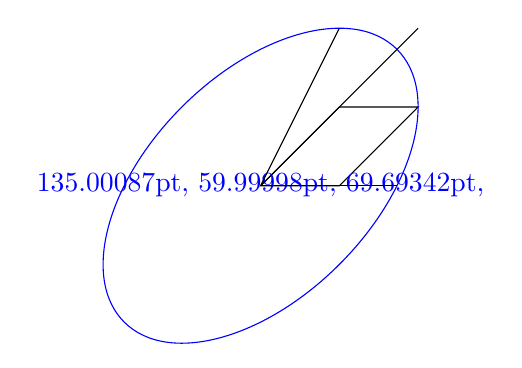
\begin{tikzpicture}[
]

\draw (0,0)coordinate(1)--(1,1)coordinate(2)--(2,1)coordinate(3)--(1,0)coordinate(4)--cycle;

\path (2)--(3)coordinate[midway](M1);
\path (3)--(4)coordinate[midway](M2);
\path (2)--(4)coordinate[midway](M);




%\draw (0,0)coordinate(1)--(2,1)coordinate(2)--(4,1)coordinate(3)--(2,0)coordinate(4)--cycle;

\pgfmathsetmacro{\st}{sqrt(3)}

\path (1,2)coordinate[](M1);
\path (\st, 0)coordinate[](M2);
\path (0,0)coordinate[](M);
\path (2,2)coordinate[](3);



\draw[blue] 
	let \p1=(M), \p2=(M1), \p3=(M2), 
	% t0 
	 \n2={.5*atan2((2*((\x3-\x1)*(\x2-\x1)+(\y3-\y1)*(\y2-\y1))),((\x3-\x1)*(\x3-\x1)+(\y3-\y1)*(\y3-\y1)-((\x2-\x1)*(\x2-\x1)+(\y2-\y1)*(\y2-\y1))))},
	% a
	 \n3={sqrt( ((\x3-\x1)*cos(\n2)+(\x2-\x1)*sin(\n2))^2 + ((\y3-\y1)*cos(\n2)+(\y2-\y1)*sin(\n2))^2)},
	% b
	 \n4={sqrt(((\x3-\x1)*cos(\n2+90)+(\x2-\x1)*sin(\n2+90))^2 + ((\y3-\y1)*cos(\n2+90)+(\y2-\y1)*sin(\n2+90))^2))},
	 % Angle
	 \n6={atan2( (\y3-\y1)*cos(\n2+90)+(\y2-\y1)*sin(\n2+90), (\x3-\x1)*cos(\n2+90)+(\x2-\x1)*sin(\n2+90)}
  in (M) ellipse [x radius=\n3, y radius=\n4,rotate=\n6+90] node{\n6, \n2, \n3, \n5};

\draw (M)--(M1);
\draw (M)--(M2);
\draw (M)--(3);


\end{tikzpicture}
\end{document}